In this section, the mobile application used to control the hydrometer will be outlined. The user will interact with the hydrometer application, which will send the request to the server.

\begin{figure}[h!]
	\centering
 	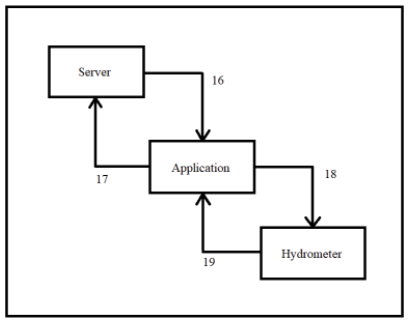
\includegraphics[width=0.60\textwidth]{images/mobile_phone_subsystem}
 \caption{Mobile Phone Subsystem}
\end{figure}

\subsection{Layer Hardware}
The phone layer will be a mobile application emulated on a physical computer operating system with the ability to connect wireless via Bluetooth to the Controller Subsystems. It will process data given to it from the Controller subsystem and transfer it to the subsystems inside the Phone Layer.

\subsection{Layer Operating System}
The physical system's Operating System emulating the Android application will be macOS Catalina version 10.15.6 and the emulated Operating System will be Android Ice Cream Sandwich version 4.0.

\subsection{Layer Software Dependencies}
The main dependency that will be operating is Android Studio and SDK tools version 4.0.1.

\subsection{Database Subsystem}
The database will be where all data on an hourly/daily basis will be stored. This data will be stored for use and analysis by the user at the time of their choosing.